\documentclass[relatorio]{inf-ufg}
% Op��es da classe inf-ufg (ao usar mais de uma, separe por vi�rgulas)
%   [tese]         -> Tese de doutorado.
%   [dissertacao]  -> Disserta��o de mestrado (padr�o).
%   [monografia]   -> Monografia de especializa��o.
%   [relatorio]    -> Relat�rio final de gradua��o.
%   [abnt]         -> Usa o estilo "abnt-alf" de cita��o bibliogr�fica.
%   [nocolorlinks] -> Os links de navega��o no texto ficam na cor preta.
%                     Use esta op��o para gerar o arquivo para impress�o
%                     da vers�o final do seu texto!!!

\usepackage{placeins}
\usepackage{longtable}

\begin{document}

\autor{Ana Let�cia Herculano da Silva}
\autorR{Silva, Ana Let�cia Herculano da}

\titulo{T�cnicas e Crit�rios de Testes em uma Aplica��o de Banco de Dados Relacioanal}
\subtitulo{Estudo de Caso}

\cidade{Goi�nia}
\dia{03} %
\mes{07} % Data da apresenta��o/defesa do trabalho
\ano{2017} % Formato num�rico: \dia{01}, \mes{01} e \ano{2009}

\orientador{Dr. C�ssio Leonardo Rodrigues}
\orientadorR{Dr. Rodrigues, C�ssio Leonardo}

\coorientador{Dr. Edmundo S�rgio Spoto}
\coorientadorR{Dr. Spoto, Edmundo S�rgio}

\universidade{Universidade Federal de Goi�s}
\uni{UFG}
\unidade{Instituto de Inform�tica}

\universidadeco{ Universidade Federal de Goi�s}
\unico{UFG}
\unidadeco{Instituto de Inform�tica}

\programa{Sistemas de Informa��o}
\concentracao{Teste de Software}

%-------------------------------------------------- ELEMENTOS PR�-TEXTUAIS %
\capa    % Gera o modelo da capa externa do trabalho
\publica % Gera a autoriza��o para publicacao em formato eletronico
\rosto   % Primeira folha interna do trabalho

\begin{aprovacao}
\banca{ Nome do membro da banca}{ Unidade acad�mica\ --  Sigla da universidade}
% Use o comando \profa se o membro da banca for do sexo feminino.
\profa{ Nome do membro da banca}{ Unidade acad�mica\ --  Sigla da universidade}
\end{aprovacao}
\direitos{Graduanda em Sistemas de Informa��o na UFG - Universidade Federal de Goi�s. Durante sua gradua��o, participou do projeto de homologa��o de PAF-ECF (Programa Aplicativo Fiscal - Emissor de Cupom Fiscal), prestando consultoria em homologa��o e teste de software para empresas de todo o Brasil. Possui certifica��o CTFL (Certified Tester, Foundation Level) e atuou em empresas goianas de software, especificamente na �rea de teste de software. Possui experi�ncia com sistemas de escritura��o fiscal, documentos fiscais eletr�nicos (NF-e, CT-e e afins), GRP (Government Resource Planning) e ITSM (IT Service Management). Atualmente trabalha como Analista de Testes em um sistema voltado para glosa de conv�nios hospitalares.}


\begin{dedicatoria}
\textless Dedicat�ria do trabalho a alguma pessoa, entidade, etc.\textgreater
\end{dedicatoria}
\begin{agradecimentos}
\textless Texto com agradecimentos �quelas pessoas/entidades que, na opini�o do autor, deram alguma contribu���o relevante para o desenvolvimento do trabalho.\textgreater
\end{agradecimentos}



\epigrafe{\textless Ep�grafe � uma cita��o relacionada com o t�pico do texto\textgreater}
{\textless Nome do autor da cita��o\textgreater}
{\textless T�tulo da refer�ncia � qual a cita��o pertence\textgreater}

\chaves{\textless Palavra chave 1, palavra chave 2, etc.\textgreater}

\begin{resumo} 
\textless Resumo do trabalho\textgreater
\end{resumo}


\keys{\textless Keyword 1, keyword 2, etc.\textgreater}

\begin{abstract}{\textless Work title\textgreater}
A sketchy summary of the main points of the text.
\end{abstract}


\tabelas[figtab]


%--------------------------------------------------------------- CAPITULOS %

\chapter{Introdu��o}
\label{cap:intro}

Este documento mostra como usar o \LaTeX\ com a classe \textsf{inf-ufg} para formatar teses, disserta��es, monografias e relat�rios de conclus�o de curso, segundo o padr�o adotado pelo Instituto de Inform�tica da UFG. Este documento e a classe \textsf{inf-ufg} foram, em grande parte, copiados e adaptados da classe \textsf{thesisPUC} e do texto de Thomas Lewiner \cite{Lew2002} que descreve a sua utiliza��o.

 \LaTeX\ � um sistema de editora��o eletr�nica muito usado para produzir documentos cient�ficos de alta qualidade tipogr�fica. O sistema tamb�m � �til para produzir todos os tipos de outros documentos, desde simples cartas at� livros completos.

Se voc� precisar de algum material de apoio referente ao \LaTeX, d� uma olhada em um dos sites do Comprehensive TEX Archive Network (CTAN). O site est� em \href{http://www.ctan.org/}{www.ctan.org}. Todos os pacotes podem ser obtidos via \textsf{FTP} \href{ftp://www.ctan.org/}{ftp://www.ctan.org} e existem v�rios servidores em todo o mundo. Eles podem ser encontrados, por exemplo, em \href{ftp://ctan.tug.org/}{ftp://ctan.tug.org} (EUA), \href{ftp://ftp.dante.de/}{ftp://ftp.dante.de} (Alemanha), \href{ftp://ftp.tex.ac.uk/}{ftp://ftp.tex.ac.uk} (Reino Unido).

Voc� pode encontrar uma grande quantidade de informa��es e dicas na p�gina dos usu�rios brasileiros de \LaTeX\ (\TeX-BR). O endere�o � \href{http://biquinho.furg.br/tex-br/}{http://biquinho.furg.br/tex-br/}.
Tanto no CTAN quanto no \TeX-BR est�o dispon�veis bons documentos em portugu�s sobre o \LaTeX. Em particular no CTAN, est� dispon�vel uma introdu��o bastante completa em portugu�s: \href{http://www.ctan.org/tex-archive/info/lshort/portuguese-BR/lshortBR.pdf}{CTAN:/tex-archive/info/lshort/portuguese-BR/}. No \TeX-BR tamb�m existe um documento com exemplos de uso de \LaTeX\ e de v�rios pacotes: \href{http://biquinho.furg.br/tex-br/doc/LaTeX-demo/}{http://biquinho.furg.br/tex-br/doc/LaTeX-demo/} . O objetivo � ser, atrav�s de exemplos, um guia para o usu�rio de \LaTeX\ iniciante e intermedi�rio, podendo, ainda, servir como um guia de refer�ncia r�pida para usu�rios avan�ados.

Se voc� quer usar o \LaTeX\ em seu computador, verifique em quais sistemas ele est� dispon�vel em \href{http://www.ctan.org/tex-archive/systems/}{CTAN:/tex-archive/systems}. Em particular para \textsf{MS Windows}, o sistema gratuito \href{http://www.miktex.org/}{MikTeX}, dispon�vel no CTAN e no site \href{http://www.miktex.org/}{www.miktex.org} � completo e atualizado de todas as op��es  que voc� poderia precisar para editar o seu texto.

O estilo \textsf{inf-ufg} se integra completamente ao \LaTeXe. Uma tese, disserta��o ou monografia escrita no estilo padr�o do \LaTeX\ para teses (estilo \verb|report|) pode ser formatada em 15 minutos para se adaptar �s normas da UFG.

O estilo \textsf{inf-ufg} foi desenhado para minimizar a quantidade de texto e de comandos necess�rios para escrever a sua disserta��o. S� � preciso inserir algumas macros no in�cio do seu arquivo \LaTeX, precisando os dados bibliogr�ficos da sua disserta��o (por exemplo o seu nome, o titulo da disserta��o\ldots). Em seguida, cada p�gina dos elementos pr�-textuais ser� formatada usando macros ou ambientes espec�ficos. O corpo do texto � editado normalmente. Finalmente, as refer�ncias bibliogr�ficas podem ser entradas manualmente (via o comando \verb|\bibitem| do \LaTeX\ padr�o) ou usando o sistema BiBTeX (muito mais recomend�vel). Neste caso, os arquivos \verb|inf-ufg.bst| e \verb|abnt-alf.bst| permitem a formata��o das refer�ncias bibliogr�ficas segundo as normas da UFG.


\chapter{Teste de Software}
\label{cap:teste}

%% - - - - - - - - - - - - - - - - - - - - - - - - - - - - - - - - - - -
\section{Conceitos de Teste de Software}
\label{sec:conceitosTesteSoftware}


As op��es da classe s�o \verb|[tese]| (para tese de doutorado), \verb|[dissertacao]| (para disserta��o de mestrado), \verb|[monografia]| (para monografia de curso de especializa��o e \verb|[relatorio]| (para relat�rio final de curso de gradua��o). Se nenhuma op��o for declarada, o documento � considerado como uma disserta��o de mestrado. Se a op��o \verb|[abnt]| for utilizada, as cita��es bibliogr�ficas ser�o geradas conforme definido pelo grupo de trabalho \textsf{abnt-tex}. Contudo, o mais recomend�vel � n�o utilizar essa op��o. Com a op��o \verb|[nocolorlinks]| todos os {\em links} de navega��o no texto ficam na cor preta. O ideal � usar esta op��o para gerar o arquivo para impress�o, pois a qualidade da impress�o dos {\em links} fica superior.


%% - - - - - - - - - - - - - - - - - - - - - - - - - - - - - - - - - - -
\section{T�cnicas e Crit�rios de Teste de Software}
\label{sec:tecnicasCriteriosTesteSoftware}


%% - - - - - - - - - - - - - - - - - - - - - - - - - - - - - - - - - - -
\section{Teste Funcional}
\label{sec:testeFuncional}
Os elementos pr�--textuais s�o definidos p�gina por p�gina, conforme descritos a seguir:


%% lista!
\begin{itemize}
\item O primeiro argumento � o Perfil do aluno; e
\item O segundo argumento � a lista das palavras--chaves para a Ficha Catalogr�fica.
\end{itemize}


%% - - - - - - - - - - - - - - - - - - - - - - - - - - - - - - - - - - -
\section{Teste de Muta��o}
\label{sec:testeMutacao}

X-Man


%% - - - - - - - - - - - - - - - - - - - - - - - - - - - - - - - - - - -
\section{Banco de Dados}
\label{sec:bancoDeDados}
\chapter{Banco de Dados}
\label{cap:bancoDeDados}

Atualmente todas as empresas que utilizam algum software para administra��o de seus neg�cios precisam manter seus dados armazenados e protegidos de alguma maneira. O acesso a esses dados muitas vezes necessitam de agilidade e confiabilidade, para quem o utiliza. 

Elmasri e Navathe (2005)\cite{ElmasriNavathe}, explicam que Banco de Dados � uma cole��o de dados com relacionados, ele � projetado, constru�do e s�o inseridos dados nele. Os dados s�o fatos que podem ser gravados e possui um significado impl�cito. O Banco de Dados pode ser de qualquer tamanho e sua complexidade pode ser vari�vel.  
Um sistema gerenciador de banco de dados (SGBD) � uma cole��o de programas que permite ao usu�rio criar, acessar e modificar esses programas. Ele facilita a defini��o, constru��o, manipula��o e compartilhamento do BD entre aplica��es e usu�rios diversos. Algumas fun��es importantes de um SGBD � a prote��o do sistema com rela��o � falhas, funcionamento e tipos de acessos n�o autorizados e tamb�m a manuten��o do BD (Elmasri; Navathe, 2005)\cite{ElmasriNavathe}).

Em 1970 Edgar Frank Codd\cite{Codd1970}, da IBM, publicou um artigo sobre o modelo relacional baseado em �lgebra relacional e c�lculos matem�ticos, mas somente na d�cada de 80 esse modelo foi disponibilizado, era o Oracle e o SQL/DS (Structured Query Language/Data System) da IBM (International Business Machines). Hoje em dia existem outros tipos de modelo relacional da Oracle, IBM e Microsoft. O SQL/DS atualmente � o DB2 da IBM, o Oracle, o Access da Microsoft, entre outros (Elmasri; Navathe, 2005)\cite{ElmasriNavathe}. 

Segundo Spoto(2000)\cite{Spoto} O modelo relacional representa uma base de dados como uma cole��o de rela��es. Informalmente, cada rela��o pode ser considerada como uma tabela. Existem importantes diferen�as entre rela��es e arquivos; a principal delas � a forma��o estruturada de seus componentes. Quando uma rela��o � tratada como uma tabela de valores, cada linha na tabela representa uma cole��o de valores de dados relacionados. Esses valores podem ser  interpretados como fatos que representam uma entidade do mundo real ou um relacionamento. O nome da tabela e os nomes das colunas s�o usados para ajudar a interpretar os valores em cada linha da tabela. Por exemplo, uma tabela com nome \verb|EMPLOYEE| armazena valores relacionados aos empregados de uma empresa, onde cada linha cont�m os dados sobre um determinado empregado. Os nomes das colunas \verb|emp_id|, \verb|emp_fname|, e \verb|emp_lname| interpretam os valores de dados espec�ficos para cada linha,baseados nos valores de cada coluna. Todos os valores de uma coluna devem ser do mesmo tipo de dados.

No modelo relacional existem quatro termos que s�o utilizados, dom�nio, tupla, atributo e rela��o.  Alguns autores definem um dom�nio D, como um conjunto de valores at�micos, sendo a menor unidade de dado e individual no Modelo Relacional (Elmasri; Navathe, 2005)\cite{ElmasriNavathe}. Portanto, um dom�nio � um conjunto de tais valores, todos do mesmo tipo, pois para cada atributo existe um conjunto de valores permitidos, que � o dom�nio desse atributo (Souza, 2008)

Outra defini��o a se destacar � de uma rela��o. Uma Rela��o  \verb|R (A1, A2, A3, .., An)|, o elemento A1 refere-se aos atributos de uma rela��o, que  � o nome do papel desempenhado por um dom�nio D. Uma rela��o R (A1, A2, A3, .., An), indicada por r(R) � um conjunto de v�rias tuplas r{t1,t2,...tn}. Cada n-tuplas � uma lista ordenada de n valores, cada valor � um elemento do dom�nio  (A) ou um valor \verb|null| (Elmasri; Navathe, 2005)\cite{ElmasriNavathe}.    


%% figura 1
\begin{figure}[H]
	\centering
	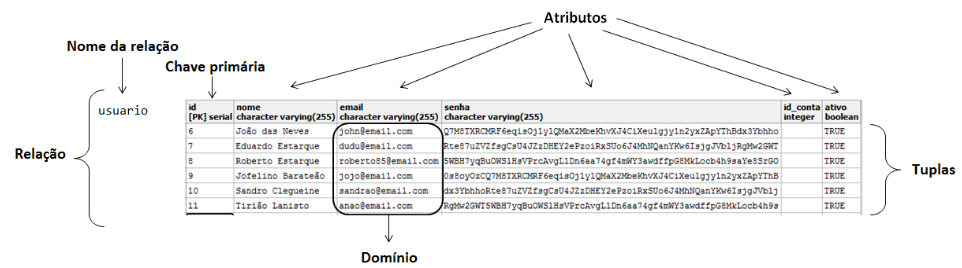
\includegraphics[width=0.9\textwidth]{./fig/figura1}
	\caption{Principais elementos de uma rela��o}
	\label{fig:figura1}
\end{figure}


As chaves em um modelo de BD relacionais s�o importantes, pois s�o elas que distinguem unicamente uma tupla na rela��o, ou seja, nenhum par de tupla pode ter o mesmo valor para todos os atributos. S�o atributos que podem ser nomeados como super-chave, candidata, prim�ria e estrangeira, e, caracterizam-se como uma propriedade da rela��o inteira, e n�o das tuplas individuais (Silberschatz et al., 2006)\cite{Silberschatz}.

% - - - - - - - - - - - - - - - - - - - - - - - - - - - - - - - - - - -
\section{Restri��es de Banco de Dados}
\label{sec:restricoesBd} 

\subsection{Restri��es de Dom�nio}
\label{restricoesDominio}

\subsection{Restri��es de Integridade Sem�ntica}
\label{restricoesIntegridadeSemantica}

\subsection{Restri��es de Integridade Referencial e de Chave Prim�ria}
\label{restricoesIntegridadeReferencial}

% - - - - - - - - - - - - - - - - - - - - - - - - - - - - - - - - - - -
\section{Aplica��es de Banco de Dados}
\label{sec:aplicacoesBd} 

% - - - - - - - - - - - - - - - - - - - - - - - - - - - - - - - - - - -
\section{Linguagem de Banco de Dados}
\label{sec:linguagemBd} 






\chapter{Introdu��o}
\label{cap:intro}

Este documento mostra como usar o \LaTeX\ com a classe \textsf{inf-ufg} para formatar teses, disserta��es, monografias e relat�rios de conclus�o de curso, segundo o padr�o adotado pelo Instituto de Inform�tica da UFG. Este documento e a classe \textsf{inf-ufg} foram, em grande parte, copiados e adaptados da classe \textsf{thesisPUC} e do texto de Thomas Lewiner \cite{Lew2002} que descreve a sua utiliza��o.

 \LaTeX\ � um sistema de editora��o eletr�nica muito usado para produzir documentos cient�ficos de alta qualidade tipogr�fica. O sistema tamb�m � �til para produzir todos os tipos de outros documentos, desde simples cartas at� livros completos.

Se voc� precisar de algum material de apoio referente ao \LaTeX, d� uma olhada em um dos sites do Comprehensive TEX Archive Network (CTAN). O site est� em \href{http://www.ctan.org/}{www.ctan.org}. Todos os pacotes podem ser obtidos via \textsf{FTP} \href{ftp://www.ctan.org/}{ftp://www.ctan.org} e existem v�rios servidores em todo o mundo. Eles podem ser encontrados, por exemplo, em \href{ftp://ctan.tug.org/}{ftp://ctan.tug.org} (EUA), \href{ftp://ftp.dante.de/}{ftp://ftp.dante.de} (Alemanha), \href{ftp://ftp.tex.ac.uk/}{ftp://ftp.tex.ac.uk} (Reino Unido).

Voc� pode encontrar uma grande quantidade de informa��es e dicas na p�gina dos usu�rios brasileiros de \LaTeX\ (\TeX-BR). O endere�o � \href{http://biquinho.furg.br/tex-br/}{http://biquinho.furg.br/tex-br/}.
Tanto no CTAN quanto no \TeX-BR est�o dispon�veis bons documentos em portugu�s sobre o \LaTeX. Em particular no CTAN, est� dispon�vel uma introdu��o bastante completa em portugu�s: \href{http://www.ctan.org/tex-archive/info/lshort/portuguese-BR/lshortBR.pdf}{CTAN:/tex-archive/info/lshort/portuguese-BR/}. No \TeX-BR tamb�m existe um documento com exemplos de uso de \LaTeX\ e de v�rios pacotes: \href{http://biquinho.furg.br/tex-br/doc/LaTeX-demo/}{http://biquinho.furg.br/tex-br/doc/LaTeX-demo/} . O objetivo � ser, atrav�s de exemplos, um guia para o usu�rio de \LaTeX\ iniciante e intermedi�rio, podendo, ainda, servir como um guia de refer�ncia r�pida para usu�rios avan�ados.

Se voc� quer usar o \LaTeX\ em seu computador, verifique em quais sistemas ele est� dispon�vel em \href{http://www.ctan.org/tex-archive/systems/}{CTAN:/tex-archive/systems}. Em particular para \textsf{MS Windows}, o sistema gratuito \href{http://www.miktex.org/}{MikTeX}, dispon�vel no CTAN e no site \href{http://www.miktex.org/}{www.miktex.org} � completo e atualizado de todas as op��es  que voc� poderia precisar para editar o seu texto.

O estilo \textsf{inf-ufg} se integra completamente ao \LaTeXe. Uma tese, disserta��o ou monografia escrita no estilo padr�o do \LaTeX\ para teses (estilo \verb|report|) pode ser formatada em 15 minutos para se adaptar �s normas da UFG.

O estilo \textsf{inf-ufg} foi desenhado para minimizar a quantidade de texto e de comandos necess�rios para escrever a sua disserta��o. S� � preciso inserir algumas macros no in�cio do seu arquivo \LaTeX, precisando os dados bibliogr�ficos da sua disserta��o (por exemplo o seu nome, o titulo da disserta��o\ldots). Em seguida, cada p�gina dos elementos pr�-textuais ser� formatada usando macros ou ambientes espec�ficos. O corpo do texto � editado normalmente. Finalmente, as refer�ncias bibliogr�ficas podem ser entradas manualmente (via o comando \verb|\bibitem| do \LaTeX\ padr�o) ou usando o sistema BiBTeX (muito mais recomend�vel). Neste caso, os arquivos \verb|inf-ufg.bst| e \verb|abnt-alf.bst| permitem a formata��o das refer�ncias bibliogr�ficas segundo as normas da UFG.


\chapter{Descri��o da classe \textsf{inf-ufg}}
\label{cap:descr}

%% - - - - - - - - - - - - - - - - - - - - - - - - - - - - - - - - - - -
\section{Op��es da classe}
\label{sec:opcoes}
Para usar esta classe num documento \LaTeXe, coloque os arquivos 
\verb|inf-ufg.cls|,\ \verb|inf-ufg.bst|,\ \verb|abnt-num.bst|,\ \verb|atbeginend.sty|\ e \verb|tocloft.sty|\ numa pasta onde o compilador \LaTeX\ pode ach�--lo (normalmente na mesma pasta que seu arquivo \verb|.tex|), e defina--o como o estilo do seu documento. Por exemplo, uma disserta��o de mestrado que usa o modelo abnt de cita��es bibliogr�ficas:
\begin{verbatim}
\documentclass[dissertacao,abnt]{inf-ufg}
...
\begin{document}
\end{verbatim}

As op��es da classe s�o \verb|[tese]| (para tese de doutorado), \verb|[dissertacao]| (para disserta��o de mestrado), \verb|[monografia]| (para monografia de curso de especializa��o e \verb|[relatorio]| (para relat�rio final de curso de gradua��o). Se nenhuma op��o for declarada, o documento � considerado como uma disserta��o de mestrado. Se a op��o \verb|[abnt]| for utilizada, as cita��es bibliogr�ficas ser�o geradas conforme definido pelo grupo de trabalho \textsf{abnt-tex}. Contudo, o mais recomend�vel � n�o utilizar essa op��o. Com a op��o \verb|[nocolorlinks]| todos os {\em links} de navega��o no texto ficam na cor preta. O ideal � usar esta op��o para gerar o arquivo para impress�o, pois a qualidade da impress�o dos {\em links} fica superior.


%% - - - - - - - - - - - - - - - - - - - - - - - - - - - - - - - - - - -
\section{Par�metros da classe}
\label{sec:param}
Os elementos pr�-textuais s�o definidos p�gina por p�gina e dependem da correta defini��o dos par�metros listados a seguir (aqueles que cont�m um texto/valor padr�o n�o precisam ser definidos, caso atenda a situa��o do autor do texto que est� usando a classe \verb|inf-ufg.cls|):

% \setlength{\topsep}{5.2em}
 \begin{itemize}%\addtolength{\itemsep}{-0.7em}
\item \verb|\autor| : Nome completo do autor da tese, come�ando pelo apelido (ex.: Jos� da Silva);
\item \verb|\autorR| : Nome completo do autor da tese, come�ando pelo nome (ex.: da Silva, Jos�);
\item \verb|\titulo| : T�tulo da tese, disserta��o, monografia ou relat�rio de conclus�o de curso;
\item \verb|\subtitulo| : Se tiver um subt�tulo, use este macro para defini--lo;

\item \verb|\cidade| : A cidade de edi��o. A cidade padr�o � \textsf{Goi�nia}.
\item \verb|\dia| : Dia do m�s da data de defesa (1--31);
\item \verb|\mes| : M�s da data de defesa (1--12);
\item \verb|\ano| : Ano da data de defesa;

\item \verb|\universidade| : Nome completo da universidade. O nome padr�o � \textsf{Universidade Federal de Goi�s};
\item \verb|\uni| : Sigla da universidade. A sigla padr�o � \textsf{UFG};
\item \verb|\unidade| : Nome da unidade acad�mica. O padr�o � \textsf{Instituto de Inform�tica};
\item \verb|\departamento| : Nome do departamento, com mai�scula na primeira letra (para o caso de unidades com mais de um departamento);

\item \verb|\programa| : Nome do programa de p�s-gradua��o, com mai�scula na primeira letra. O padr�o � \textsf{Computa��o};
\item \verb|\concentracao| : Nome da �rea de concentra��o;

\item \verb|\orientador| : Nome completo do orientador, come�ando pelo apelido;
\item \verb|\orientadorR| : Nome completo do orientador, come�ando pelo nome;

\item \verb|\orientadora| : Nome completo da orientadora, come�ando pelo apelido; use este comando e o pr�ximo se for orientadora e nao orientador.
\item \verb|\orientadoraR| : Nome completo do orientadora, come�ando pelo nome;

% \item \verb|\CDU| : CDU das publica��es do instituto (a perguntar na biblioteca central);
% \item \verb|\paginaspre| : N�mero de p�ginas pr�-textuais;
% \item \verb|\paginastex| : N�mero de p�ginas textuais;
% \item \verb|\altura| : Altura do papel utilizado para a impress�o do trabalho. O padr�o � o papel A4, de altura 29.7cm;

\item \verb|\coorientador| : Nome completo do co--orientador, come�ando pelo apelido;
\item \verb|\coorientadorR| : Nome completo do co--orientador, come�ando pelo nome;

\item \verb|\coorientadora| : Nome completo da coorientadora, come�ando pelo apelido; use este comando e o pr�ximo se for coorientadora e nao coorientador.
\item \verb|\coorientadoraR| : Nome completo do coorientadora, come�ando pelo nome;

\item \verb|\universidadeco| : Nome da universidade do coorientador;
\item \verb|\unico| : Sigla da universidade do coorientador;
\item \verb|\unidadeco| : Nome da unidade acad�mica do coorientador.\footnote{Se n�o tiver um co--orientador, n�o defina esses �ltimos sete par�metros.}
\end{itemize}

%% - - - - - - - - - - - - - - - - - - - - - - - - - - - - - - - - - - -
\section{Elementos Pr�--Textuais}
\label{sec:pre}
Os elementos pr�--textuais s�o definidos p�gina por p�gina, conforme descritos a seguir:

\paragraph{capa\\}
\verb|\capa| : Gera o modelo da capa externa do trabalho. Esta p�gina servir� apenas como modelo para a encaderna��o da vers�o final do texto. Nenhum dado � necess�rio.

\paragraph{publica��o\\}
\verb|\publica| : Gera a autoriza��o para publica��o do trabalho em formato eletr�nico e disponibiliza��o do mesmo na biblioteca virtual da UFG.

\paragraph{rosto\\}
\verb|\rosto| : Gera a folha de rosto, a qual � a primeira folha interna do trabalho. Nenhum dado � necess�rio.

\paragraph{aprova��o\\}
\verb|\aprovacao| : ambiente para a reprodu��o do termo de aprova��o da Banca Examinadora da tese ou disserta��o.

\paragraph{banca\\}
\verb|\banca| : Entrada para o nome dos examinadores, exceto o(s) orientador(es).

\noindent\verb|\profa| : Entrada para o nome das examinadoras, exceto o(s) orientador(es).

\paragraph{direitos\\}
\verb|\direitos| : Macro com 2 argumentos para gerar os direitos autorais, o perfil do aluno e a ficha catalogr�fica da Biblioteca Central da UFG.
\begin{itemize}
\item O primeiro argumento � o Perfil do aluno; e
\item O segundo argumento � a lista das palavras--chaves para a Ficha Catalogr�fica.
\end{itemize}

\paragraph{dedicat�ria\\}
\verb|\dedicatoria| : ambiente para escrever a dedicat�ria. � poss�vel trocar o espa�amento dentro desse ambiente do mesmo jeito que no \LaTeX\ padr�o.

\paragraph{agradecimentos\\}
\verb|\agradecimentos| : ambiente para escrever os agradecimentos. � poss�vel trocar o espa�amento dentro desse ambiente do mesmo jeito que no \LaTeX\ padr�o.

\paragraph{resumo\\}
\verb|\chaves| : A lista das palavras chaves, separadas por `;'. Deve ser definido antes do ambiente \verb|\resumo|, o qual � usado para escrever o resumo em portugu�s.

\paragraph{abstract\\}
\verb|\keys| : A lista das palavras chaves em ingl�s, separadas por `;'. Deve ser definido antes do ambiente \verb|\abstract|, o qual cont�m 1 argumento e � usado escrever o resumo em ingl�s. O argumento deve ser o t�tulo do trabalho em ingl�s.

\paragraph{tabelas\\}
\verb|\tabelas| : Macro com 1 argumento opcional para gerar as tabelas. O argumento pode ser:
\begin{itemize}
 \item nada [] : gera apenas o sum�rio;
 \item \textsf{fig} : gera o sum�rio e uma lista de figuras;
 \item \textsf{tab} : gera o sum�rio e uma lista de tabelas;
 \item \textsf{alg} : gera o sum�rio e uma lista de algoritmos;
 \item \textsf{cod} : gera o sum�rio e uma lista de programas.
% \item \textsf{figtab} : gera o sum�rio, uma lista de tabelas, e uma lista de figuras;
% \item \textsf{figtabalg} : gera o sum�rio e listas de tabelas, de figuras e de algoritmos;
% \item \textsf{figtabalgcod} : gera o sum�rio e listas de tabelas, de figuras, de algoritmos e de programas;
% \item (qualquer outra coisa) : gera somente o sum�rio.
\end{itemize}

Pode-se usar qualquer combina��o dessas op��es. Por exemplo:
\begin{itemize}
 \item \textsf{figtab} : gera o sum�rio e listas de figuras e tabelas,
 \item \textsf{figtabcod} : gera o sum�rio e listas de figuras, tabelas e c�digos de programas;
 \item \textsf{figtabalg} : gera o sum�rio e listas de figuras, tabelas e algoritmos;
 \item \textsf{figtabalgcod} : gera o sum�rio e listas de figuras, tabelas, algoritmos e c�digos de programas
\end{itemize}

\paragraph{ep�grafe\\}
\verb|\epigrafe| : Macro com 3 argumentos que permite editar um ep�grafe. O primeiro argumento � o texto da cita��o. O segundo argumento � o nome do autor da cita��o. O terceiro argumento � o t�tulo da refer�ncia � qual a cita��o pertence.

\chapter{Plano de Teste}
\label{planoTeste}



% - - - - - - - - - - - - - - - - - - - - - - - - - - - - - - - - - - -
\section{Plano de Testes Baseado no Teste Funcional em BDR}
\label{planoTestesBDR}

\subsection{Testes Intra - Tabelas}
\label{testesIntraTabela}

\subsection{Testes Inter - Tabelas}
\label{testesInterTabela}
\chapter{Resultados obtidos}
\label{resultados}

\chapter{Conclusão e trabalhos futuros}
\label{conclusao}

%------------------------------------------------------------ BIBLIOGRAFIA %
\cleardoublepage
\nocite{*} %%% Retire esta linha para gerar a bibliografia com apenas as
           %%% refer�ncias usadas no seu texto!
\arial
\bibliography{./bib/modelo-tese} %%% Nomes dos seus arquivos .bib
\label{ref-bib}

%--------------------------------------------------------------- AP�NDICES %
\apendices

\chapter{Script de cria��o da base de dados}
\label{apend:A}
Ap�ndicess s�o iniciados com o comando \verb|\apendices|.
\chapter{Exemplo de Outro Ap�ndice}
\label{apend:2}
Texto do Ap�ndice~\ref{apend:2}.

Ap�ndices s�o iniciados com o comando \verb|\apendices|.
Ap�ndices s�o iniciados com o comando \verb|\apendices|.
Ap�ndices s�o iniciados com o comando \verb|\apendices|.
Ap�ndices s�o iniciados com o comando \verb|\apendices|.
Ap�ndices s�o iniciados com o comando \verb|\apendices|.
Ap�ndices s�o iniciados com o comando \verb|\apendices|.
Ap�ndices s�o iniciados com o comando \verb|\apendices|.
Ap�ndices s�o iniciados com o comando \verb|\apendices|.
Ap�ndices s�o iniciados com o comando \verb|\apendices|.
Ap�ndices s�o iniciados com o comando \verb|\apendices|.
Ap�ndices s�o iniciados com o comando \verb|\apendices|.
Ap�ndices s�o iniciados com o comando \verb|\apendices|.
Ap�ndices s�o iniciados com o comando \verb|\apendices|.
Ap�ndices s�o iniciados com o comando \verb|\apendices|.
Ap�ndices s�o iniciados com o comando \verb|\apendices|.
Ap�ndices s�o iniciados com o comando \verb|\apendices|.

Ap�ndices s�o iniciados com o comando \verb|\apendices|.
Ap�ndices s�o iniciados com o comando \verb|\apendices|.
Ap�ndices s�o iniciados com o comando \verb|\apendices|.
Ap�ndices s�o iniciados com o comando \verb|\apendices|.
Ap�ndices s�o iniciados com o comando \verb|\apendices|.
Ap�ndices s�o iniciados com o comando \verb|\apendices|.
Ap�ndices s�o iniciados com o comando \verb|\apendices|.
Ap�ndices s�o iniciados com o comando \verb|\apendices|.
Ap�ndices s�o iniciados com o comando \verb|\apendices|.
Ap�ndices s�o iniciados com o comando \verb|\apendices|.
Ap�ndices s�o iniciados com o comando \verb|\apendices|.
Ap�ndices s�o iniciados com o comando \verb|\apendices|.

Ap�ndices s�o iniciados com o comando \verb|\apendices|.
Ap�ndices s�o iniciados com o comando \verb|\apendices|.
Ap�ndices s�o iniciados com o comando \verb|\apendices|.
Ap�ndices s�o iniciados com o comando \verb|\apendices|.
Ap�ndices s�o iniciados com o comando \verb|\apendices|.
Ap�ndices s�o iniciados com o comando \verb|\apendices|.
Ap�ndices s�o iniciados com o comando \verb|\apendices|.
Ap�ndices s�o iniciados com o comando \verb|\apendices|.
Ap�ndices s�o iniciados com o comando \verb|\apendices|.
Ap�ndices s�o iniciados com o comando \verb|\apendices|.
Ap�ndices s�o iniciados com o comando \verb|\apendices|.
Ap�ndices s�o iniciados com o comando \verb|\apendices|.
Ap�ndices s�o iniciados com o comando \verb|\apendices|.
Ap�ndices s�o iniciados com o comando \verb|\apendices|.

Ap�ndices s�o iniciados com o comando \verb|\apendices|.
Ap�ndices s�o iniciados com o comando \verb|\apendices|.
Ap�ndices s�o iniciados com o comando \verb|\apendices|.
Ap�ndices s�o iniciados com o comando \verb|\apendices|.
Ap�ndices s�o iniciados com o comando \verb|\apendices|.
Ap�ndices s�o iniciados com o comando \verb|\apendices|.
Ap�ndices s�o iniciados com o comando \verb|\apendices|.
Ap�ndices s�o iniciados com o comando \verb|\apendices|.
Ap�ndices s�o iniciados com o comando \verb|\apendices|.
Ap�ndices s�o iniciados com o comando \verb|\apendices|.
Ap�ndices s�o iniciados com o comando \verb|\apendices|.
Ap�ndices s�o iniciados com o comando \verb|\apendices|.
Ap�ndices s�o iniciados com o comando \verb|\apendices|.
Ap�ndices s�o iniciados com o comando \verb|\apendices|.

Ap�ndices s�o iniciados com o comando \verb|\apendices|.
Ap�ndices s�o iniciados com o comando \verb|\apendices|.
Ap�ndices s�o iniciados com o comando \verb|\apendices|.
Ap�ndices s�o iniciados com o comando \verb|\apendices|.
Ap�ndices s�o iniciados com o comando \verb|\apendices|.
Ap�ndices s�o iniciados com o comando \verb|\apendices|.
Ap�ndices s�o iniciados com o comando \verb|\apendices|.
Ap�ndices s�o iniciados com o comando \verb|\apendices|.
Ap�ndices s�o iniciados com o comando \verb|\apendices|.
Ap�ndices s�o iniciados com o comando \verb|\apendices|.
Ap�ndices s�o iniciados com o comando \verb|\apendices|.
Ap�ndices s�o iniciados com o comando \verb|\apendices|.
Ap�ndices s�o iniciados com o comando \verb|\apendices|.
Ap�ndices s�o iniciados com o comando \verb|\apendices|.

Ap�ndices s�o iniciados com o comando \verb|\apendices|.
Ap�ndices s�o iniciados com o comando \verb|\apendices|.
Ap�ndices s�o iniciados com o comando \verb|\apendices|.
Ap�ndices s�o iniciados com o comando \verb|\apendices|.
Ap�ndices s�o iniciados com o comando \verb|\apendices|.
Ap�ndices s�o iniciados com o comando \verb|\apendices|.
Ap�ndices s�o iniciados com o comando \verb|\apendices|.
Ap�ndices s�o iniciados com o comando \verb|\apendices|.
Ap�ndices s�o iniciados com o comando \verb|\apendices|.
Ap�ndices s�o iniciados com o comando \verb|\apendices|.
Ap�ndices s�o iniciados com o comando \verb|\apendices|.
Ap�ndices s�o iniciados com o comando \verb|\apendices|.
Ap�ndices s�o iniciados com o comando \verb|\apendices|.
Ap�ndices s�o iniciados com o comando \verb|\apendices|.

Ap�ndices s�o iniciados com o comando \verb|\apendices|.
Ap�ndices s�o iniciados com o comando \verb|\apendices|.
Ap�ndices s�o iniciados com o comando \verb|\apendices|.
Ap�ndices s�o iniciados com o comando \verb|\apendices|.
Ap�ndices s�o iniciados com o comando \verb|\apendices|.
Ap�ndices s�o iniciados com o comando \verb|\apendices|.
Ap�ndices s�o iniciados com o comando \verb|\apendices|.
Ap�ndices s�o iniciados com o comando \verb|\apendices|.
Ap�ndices s�o iniciados com o comando \verb|\apendices|.
Ap�ndices s�o iniciados com o comando \verb|\apendices|.
Ap�ndices s�o iniciados com o comando \verb|\apendices|.
Ap�ndices s�o iniciados com o comando \verb|\apendices|.
Ap�ndices s�o iniciados com o comando \verb|\apendices|.
Ap�ndices s�o iniciados com o comando \verb|\apendices|.

Ap�ndices s�o iniciados com o comando \verb|\apendices|.
Ap�ndices s�o iniciados com o comando \verb|\apendices|.
Ap�ndices s�o iniciados com o comando \verb|\apendices|.
Ap�ndices s�o iniciados com o comando \verb|\apendices|.
Ap�ndices s�o iniciados com o comando \verb|\apendices|.
Ap�ndices s�o iniciados com o comando \verb|\apendices|.
Ap�ndices s�o iniciados com o comando \verb|\apendices|.
Ap�ndices s�o iniciados com o comando \verb|\apendices|.
Ap�ndices s�o iniciados com o comando \verb|\apendices|.
Ap�ndices s�o iniciados com o comando \verb|\apendices|.
Ap�ndices s�o iniciados com o comando \verb|\apendices|.
Ap�ndices s�o iniciados com o comando \verb|\apendices|.
Ap�ndices s�o iniciados com o comando \verb|\apendices|.
Ap�ndices s�o iniciados com o comando \verb|\apendices|.

Ap�ndices s�o iniciados com o comando \verb|\apendices|.
Ap�ndices s�o iniciados com o comando \verb|\apendices|.
Ap�ndices s�o iniciados com o comando \verb|\apendices|.
Ap�ndices s�o iniciados com o comando \verb|\apendices|.
Ap�ndices s�o iniciados com o comando \verb|\apendices|.
Ap�ndices s�o iniciados com o comando \verb|\apendices|.
Ap�ndices s�o iniciados com o comando \verb|\apendices|.
Ap�ndices s�o iniciados com o comando \verb|\apendices|.
Ap�ndices s�o iniciados com o comando \verb|\apendices|.
Ap�ndices s�o iniciados com o comando \verb|\apendices|.
Ap�ndices s�o iniciados com o comando \verb|\apendices|.
Ap�ndices s�o iniciados com o comando \verb|\apendices|.
Ap�ndices s�o iniciados com o comando \verb|\apendices|.
Ap�ndices s�o iniciados com o comando \verb|\apendices|.

Ap�ndices s�o iniciados com o comando \verb|\apendices|.
Ap�ndices s�o iniciados com o comando \verb|\apendices|.
Ap�ndices s�o iniciados com o comando \verb|\apendices|.
Ap�ndices s�o iniciados com o comando \verb|\apendices|.
Ap�ndices s�o iniciados com o comando \verb|\apendices|.
Ap�ndices s�o iniciados com o comando \verb|\apendices|.
Ap�ndices s�o iniciados com o comando \verb|\apendices|.
Ap�ndices s�o iniciados com o comando \verb|\apendices|.
Ap�ndices s�o iniciados com o comando \verb|\apendices|.
Ap�ndices s�o iniciados com o comando \verb|\apendices|.
Ap�ndices s�o iniciados com o comando \verb|\apendices|.
Ap�ndices s�o iniciados com o comando \verb|\apendices|.
Ap�ndices s�o iniciados com o comando \verb|\apendices|.
Ap�ndices s�o iniciados com o comando \verb|\apendices|.

Ap�ndices s�o iniciados com o comando \verb|\apendices|.
Ap�ndices s�o iniciados com o comando \verb|\apendices|.
Ap�ndices s�o iniciados com o comando \verb|\apendices|.
Ap�ndices s�o iniciados com o comando \verb|\apendices|.
Ap�ndices s�o iniciados com o comando \verb|\apendices|.
Ap�ndices s�o iniciados com o comando \verb|\apendices|.
Ap�ndices s�o iniciados com o comando \verb|\apendices|.
Ap�ndices s�o iniciados com o comando \verb|\apendices|.
Ap�ndices s�o iniciados com o comando \verb|\apendices|.
Ap�ndices s�o iniciados com o comando \verb|\apendices|.
Ap�ndices s�o iniciados com o comando \verb|\apendices|.
Ap�ndices s�o iniciados com o comando \verb|\apendices|.
Ap�ndices s�o iniciados com o comando \verb|\apendices|.
Ap�ndices s�o iniciados com o comando \verb|\apendices|.

Ap�ndices s�o iniciados com o comando \verb|\apendices|.
Ap�ndices s�o iniciados com o comando \verb|\apendices|.
Ap�ndices s�o iniciados com o comando \verb|\apendices|.
Ap�ndices s�o iniciados com o comando \verb|\apendices|.
Ap�ndices s�o iniciados com o comando \verb|\apendices|.
Ap�ndices s�o iniciados com o comando \verb|\apendices|.
Ap�ndices s�o iniciados com o comando \verb|\apendices|.
Ap�ndices s�o iniciados com o comando \verb|\apendices|.
Ap�ndices s�o iniciados com o comando \verb|\apendices|.
Ap�ndices s�o iniciados com o comando \verb|\apendices|.
Ap�ndices s�o iniciados com o comando \verb|\apendices|.
Ap�ndices s�o iniciados com o comando \verb|\apendices|.
Ap�ndices s�o iniciados com o comando \verb|\apendices|.
Ap�ndices s�o iniciados com o comando \verb|\apendices|.

Ap�ndices s�o iniciados com o comando \verb|\apendices|.
Ap�ndices s�o iniciados com o comando \verb|\apendices|.
Ap�ndices s�o iniciados com o comando \verb|\apendices|.
Ap�ndices s�o iniciados com o comando \verb|\apendices|.
Ap�ndices s�o iniciados com o comando \verb|\apendices|.
Ap�ndices s�o iniciados com o comando \verb|\apendices|.
Ap�ndices s�o iniciados com o comando \verb|\apendices|.
Ap�ndices s�o iniciados com o comando \verb|\apendices|.
Ap�ndices s�o iniciados com o comando \verb|\apendices|.
Ap�ndices s�o iniciados com o comando \verb|\apendices|.
Ap�ndices s�o iniciados com o comando \verb|\apendices|.
Ap�ndices s�o iniciados com o comando \verb|\apendices|.
Ap�ndices s�o iniciados com o comando \verb|\apendices|.
Ap�ndices s�o iniciados com o comando \verb|\apendices|.

Ap�ndices s�o iniciados com o comando \verb|\apendices|.
Ap�ndices s�o iniciados com o comando \verb|\apendices|.
Ap�ndices s�o iniciados com o comando \verb|\apendices|.
Ap�ndices s�o iniciados com o comando \verb|\apendices|.
Ap�ndices s�o iniciados com o comando \verb|\apendices|.
Ap�ndices s�o iniciados com o comando \verb|\apendices|.
Ap�ndices s�o iniciados com o comando \verb|\apendices|.
Ap�ndices s�o iniciados com o comando \verb|\apendices|.
Ap�ndices s�o iniciados com o comando \verb|\apendices|.
Ap�ndices s�o iniciados com o comando \verb|\apendices|.
Ap�ndices s�o iniciados com o comando \verb|\apendices|.
Ap�ndices s�o iniciados com o comando \verb|\apendices|.
Ap�ndices s�o iniciados com o comando \verb|\apendices|.
Ap�ndices s�o iniciados com o comando \verb|\apendices|.

\chapter{Scripts dos casos de testes}
\label{apend:C}
Texto do Apêndice~\ref{apend:C}.
\chapter{Scripts dos Testes de  Mutantes}
\label{apend:D}
Texto do Apêndice~\ref{apend:C}.


\end{document}